% a longer version of this was submitted for the ngVLA project as a memo.

%  http://ngvla.nrao.edu/page/memos
%  https://library.nrao.edu/ngvla.shtml

\documentclass[11pt,twoside]{article}
\usepackage{asp2014}
\usepackage{graphicx}
\usepackage{float}
\usepackage{siunitx}


\aspSuppressVolSlug
\resetcounters

\bibliographystyle{asp2014}

\markboth{Teuben}{QAC}

\begin{document}

\title{ngVLA Memo No. 59: \\ QAC: Quick Array Combinations with CASA}
\author{Peter Teuben}
\affil{Astronomy Department, University of Maryland, College Park, MD, USA}

\paperauthor{Teuben~Peter}{teuben@astro.umd.edu}{0000-0003-1774-3436}{Astronomy Department}{University of Maryland}{College Park}{MD}{20742}{USA}

%\aindex{Teuben,~P.~J.}

\begin{abstract}

QAC is a simple python layer in CASA, developed to aid in writing scripts
for array (single dish and interferometric) combinations. Although
initially developed for TP2VIS, running simulations and comparing with
other array combination methods, this package turned out to be useful
for array design studies as well. Both ALMA, ngVLA and CARMA
simulations are already supported, but extending to more generic array
are planned. This memo complements ngVLA memo 54, where
QAC\footnote{this memo describes QAC as of February 2019}
was used for an array design study..


\end{abstract}

%\ooindex{CASA, ascl:1107.013} 

%\ssindex{instruments!interferometer}
%\ssindex{astronomy!radio!single-dish}
%\ssindex{packages!Common Astronomy Software Applications (CASA)}


\section{Introduction}

CASA (\citet{casa1}, \citet{casa2}) 
is a general purpose python interface to radio
astronomy software. It handles interferometric as well as single dish
data, all the way from ingestion, calibration and mapping to
analysis. Most ALMA and VLA data are now routinely processed with CASA
using a custom built pipeline.  CASA Users use object oriented
``tools'', or more classic python functions, called
``tasks'' in CASA. One can write very complex tasks this way, and in fact, the
ALMA/VLA pipeline is an example of such an interface. The QAC
interfaces we discuss in this memo were also designed with a specific
goal of testing the combination of single dish and interferometric data, and
for example are ideal for array design studies.

% The effect of adding short spacings can be dramatic.

% In a previous project, the ADMIT project had a similar challenge, but
% additional more complex boundary conditions.

The development of QAC started in 2017 with the TP2VIS project \citep{tp2vis}, to provide a
more easily programmable interface, orchestrate simulations and provide a
reproducable baseline using regressions. It can be obtained from \url{https://github.com/teuben/QAC}.

We first summarize the different methods how CASA can be extended by using your own
custum built python code, then how QAC is installed, and a typical usage. We also give a short
summary of the API, and publish a benchmark in the Appendix. Given that QAC is available
in github, you will likely find updates to QAC (and this memo) in this repository.

So why tinker with CASA. Several efforts have been going on. E.g. casanova
\footnote{\url{https://github.com/kaspervd/casanova}}



\section{Running python code in CASA}

CASA interacts with the user in an interactive python (ipython) session. For most users adding 
C++ code is a complex operation, but installing new python interfaces to ease writing CASA scripts
is usually fairly straightforward, and nowadays most users are familiar with this.
Several methods (and hybrid between these) exist
for CASA:\footnote{some of these methods are expected to become more common in CASA6}


\begin{itemize}

\item[1.] \verb+buildmytasks+

This is the native CASA method. The CASA Cookbook describes a
procedure to install new CASA tasks, but at the same time warns this
method may get deprecated. Nonetheless, this so-called
``buildmytasks'' has been used by other teams, most notably by the Nordic ARC
node\footnote{\url{https://www.oso.nordic-alma.se/software-tools.php}}. This
is typically run once inside the directory where your {\tt foo.py}, {\tt foo.xml},
and other material is present, after which the code, and documentation, gets installed
at the right place inside the CASA tree.

\footnotesize
\begin{verbatim}
    foo(1,'b',[1,2,3])
\end{verbatim}
\normalsize

\item[2.] \verb+import foo+

The traditional way a user includes software to a python based system
would be the python {\tt import} command.
This is fine for stable software, and can be installed with python's
{\tt setuptools} in CASA. In the future CASA6 one should be able to use
virtualenv to test out software like this without the need to write
into CASA's personal space. One can also consider the use of using \verb+$PYTHONPATH+
to point to the directory where {\tt foo.py} is present, but this method can
easily conflict with other installation methods (in fact, is strongly discouraged
in a CASA environment).

%      foo.bar(1,'b',[1,2,3])

\footnotesize
\begin{verbatim}
    foo.bar(1,'b',[1,2,3])
\end{verbatim}
\normalsize



\item[3.] \verb+execfile('foo.py')+

Will execute the code,  after which an API is available  (note this will not work in python3).
This is the method we used in QAC. Notice that no command line parameters can be passed into
the code.

%        foo_bar(1,'b',[1,2,3])

\footnotesize
\begin{verbatim}
    foo_bar(1,'b',[1,2,3])
\end{verbatim}
\normalsize


Incidentally, if these are combined and only one script needs to be executed and then analyzed
outside of CASA, a very efficient way it to use could be to call casa from the command line,
e.g. directly from bash (or via a Makefile):

\footnotesize
\begin{verbatim}
    % casa --nogui -c foo.py a=1 b='"b"' c='[1,2,3]' > foo.log 2&>1
\end{verbatim}
\normalsize

The overhead of setting up CASA before this script really starts work
varies a lot depending on cashing and what's in the casa init files, but can
be anywhere from 5 to 20 seconds. If many of these scripts are to be run, and each
only takes a short time, the overhead is too large, and 





\item[4.]  \verb+run foo.py p1 p2 p3+

Since CASA is essentially an ipython shell, the {\tt run} command can be used to execute
a scripting, including conveniently parsing ``command line arguments''.
This will need a parser for \verb+p1=sys.argv[1]+, \verb+p2=sys.argv[2]+, etc.
note this is an ipython interface, not python, though it's similar to
running in the unix shell \verb+python foo.py p1 p2 p3+, but note this is different
from the CASA method where local python variables can directly be set via the commandline
without the need for a parser.

\footnotesize
\begin{verbatim}
    run foo.py 1  'b'  [1,2,3]
\end{verbatim}
\normalsize

                           
\item[5.]   \verb+%run -m foo+

Runs the foo module (from sys.path). In the current CASA manipulating
{\tt sys.path} is not recommended, the arguments similar to those of not
using \verb+$PYTHONPATH+

\end{itemize}

Miles Lucas made his summer-2019 toolkit Radio Imaging Combination Analysis (RIKA)
available\footnote{\url{https://gitlab.com/mileslucas/RICA}}. He uses the 4th ({\tt run}) method.
In QAC we decided to use the 3rd ({\tt execfile}) method.


\subsection{Installing QAC}

QAC needs CASA to be installed, and the user can opt either to install a version
of CASA from within QAC, or assume a version of CASA that is present on the system, i.e. there
is a existing command called ``casa''. Since CASA startup can be controlled by
\verb+~/.casa/init.py+ we choose this file to {\tt execfile} the correct startup script,
aptly named {\tt casa.init.py} in the QAC distribution:


\begin{verbatim}
    execfile(os.environ['HOME'] + '/.casa/QAC/casa.init.py')
\end{verbatim}

\noindent
There are a few examples of common packages loaded by CASA in {\tt casa.init.py}

\section{Design Issues}

QAC needs to be lightweight, easy to install,

\begin{itemize}

\item
  Easy to install, ideally a one liner

\item
  Easy to pass parameters into functions of scripts

\item
  Consistent naming convention of functions and parameters

\item
  Procedural. Although python has great support for a object oriented
  programming style, and plenty is used under the hood in CASA, for
  this simple interface a simple procedural path was chosen.

\item
  clean vs. tclean. Although clean is formally not supported anymore, occasionally the two are compared, and
  this gives that option. See \verb+qac_clean1(t=True,t=False)+
  
\end{itemize}

The use of a script with parameters is very useful for re-use, especially if the script also defines defaults. A huge
drawback of the execfile approach is the lack to change these parameters. Add to this that execfile is not supported
in python3, is a no-brainer not to use it, or at least switch to ``run''.

execfile() sits in the same namespace.

run runs a file as a program, whihc is like 'casa -c foo.py', and needs extra to get the casa bagage.

\section{Example}

A typical usage would be

\begin{verbatim}
    % casa --nogui -c 
\end{verbatim}


\section{docs}

A typical simulation script might look as follows. Explanations follow later:

\footnotesize
\begin{verbatim}
    qac_ptr(phasecenter,"test123.ptg")
    qac_vla("test123","skymodel.fits", 4096, 0.01, ptg="test123.ptg",
            phasecenter=phasecenter)
            
    qac_clean1("test123/clean1",phasecenter=phasecenter)
\end{verbatim}
\normalsize

\section{Timing and Regression}

Because QAC deal almost exclusively with image type data, the regression test is invoked automatically
with the statistics report, if a regression string (!) is given, viz.

\footnotesize
\begin{verbatim}
r = "0.0038324084555372423 0.021439742878458009 -0.048513446003198624
     0.41929447650909424 383.60327838373536"
qac_stats(test+'/clean/tpint.image')
qac_stats(test+'/clean/tpint_4.tweak.image', r)
\end{verbatim}
\normalsize

where in the first instance only the statistics are reported, the second instance will also flag any deviations.
The numbers represent the mean, std, min, max and total flux of the image.

\section{Benchmarks}

A better supported show of QAC functionality is currently in the **test/bench.py, bench0.py** and **sky1.py** routines [March 2018]
as those were used in the
[SD2018](\url{https://github.com/teuben/sd2018}) workshop. Please note the software in that repo is not maintained anymore,
and updated versions can be found
within QAC.

\section{API}

Here we list the most important functions available in QAC, without
further details except for arguably descriptive parameter names and
defaults. The full and updated documentation can be seen online on
\url{https://github.com/teuben/QAC/blob/master/docs/qac.md}.

\footnotesize
\begin{verbatim}

## Adminstrativia

  qac_log(message, verbose=True)

  qac_version()

  qac_begin(label='QAC', log=True, plot=False)

  qac_end()

## Simulation routines

  qac_vla(project, skymodel, imsize, pixel, phasecenter, freq, cfg, ptg, noise)

  qac_alma(project, skymodel, imsize, pixel, phasecenter, freq, cycle, cfg, ptg)

  qac_noise(noise, *args, **kwargs)

  qac_clean1(project, ms, imsize, pixel, niter, weighting, startmodel, phasecenter, **line)

  qac_tp_otf(project, skymodel, dish, label, freq, template)

  qac_tp_vis(project, imagename, ptg, pixel, niter, phasecenter, rms, maxuv, nvgrp, fix,
             deconv, **line)

  qac_feather(project, highres, lowres, label, niteridx)

  qac_ssc(project, highres, lowres)

  qac_smooth(project, skymodel, label, niteridx)


## Helper routines

  qac_stats(image, test=None, eps=None, box=None, pb=None, pbcut=0.8, edge=False)

  qac_beam(im, normalized=True, chan=-1, plot=None)

  qac_tpdish(ptg, ptgfile=None)

  qac_phasecenter(im)

  qac_ptg(ptg, ptgfile=None)

  qtp_im_ptg(phasecenter, imsize, pixel, grid, im=[], rect=False, outfile=None)

  qac_summary(tp, ms=None, source=None, line=False)

  qac_math(outfile, infile1, oper, infile2)

  qac_mom(imcube, chan_rms, pb=None, pbcut=0.3, rms=None)

  qac_plot(image, channel=0, box=None, range=None, mode=0, title=None, plot=None)

  qac_flux(image, box=None, dv=1.0, plot='qac_flux.png')

  qac_fidelity(model, image, figure_mode=5, diffim=None, absdiffim=None, fidelityim=None,
               absmodelim=None, interactive=False)

\end{verbatim}
\normalsize


\section{Future}

CASA is a development project, the next
release will have a major overhaul how python and the C++ libraries
are integrated, and this will likely have some effect how QAC is
installed, although less on its API. 

\acknowledgements Jordan Turner and Sara Negussie have been patient contributers and users.
Part of QAC was developed under the ALMA development study ``TP2VIS''  (PI: Jin Koda) and
the ``ngVLA'' array combination study (ngVLA memo 54).

\bibliography{qac}

\newpage
\section*{Appendix A: Sample Code}


To run a large suite of simulations, it can be very useful to call CASA from the Unix command line,
and loop over many parameters, e.g.

\footnotesize
\begin{verbatim}
  casa --nogui -c vla1.py pixel_m=0.05 niter='[0,5000,15000]' dish=45 pdir='"exp102"' 
\end{verbatim}
\normalsize

As one of the products of the ``tp2vis'' ALMA development study (\citet{tp2vis})
we continued the development of the
Quick Array Combination (QAC) toolkit that simplifies writing some of these complex scripts. It also allow us
to use a different combination
method (feather, tp2vis, ssc etc.) with minimal changes to the simulations scripts.

As an example, consider the {\tt simplenoise} procedure to add a given noise to a simulation.
Here is the example calling {\tt qac\_vla()} twice, in the end generating a Measurement Set with
the correct 1 mJy/beam noise:

\footnotesize
\begin{verbatim}

 rms = 0.002                               #  request 2 mJy/beam RMS noise (NA)
 ms1 = qac_vla(pdir,model, noise=-rms)     #  noise<0 triggers it to compute the rms
 sn0 = qac_noise(noise,pdir+'/noise', ms1) #  get scaling factor from rms in ms1
 ms2 = qac_vla(pdir,model, noise=sn0)      #  MS that with correct "rms" in Jy/beam
\end{verbatim}
\normalsize

In the first Measurement Set a noise level is computed for a fixed 1 Jy noise per visiblity on a
zero model. The noise in the resulting dirty map, computed in {\tt qac\_noise()}, is then the scaling factor ({\tt sn0}
that needs to be applied to get the correct requested noise level in the second Measurement Set.








% figures
\newpage

\begin{figure}
\centering
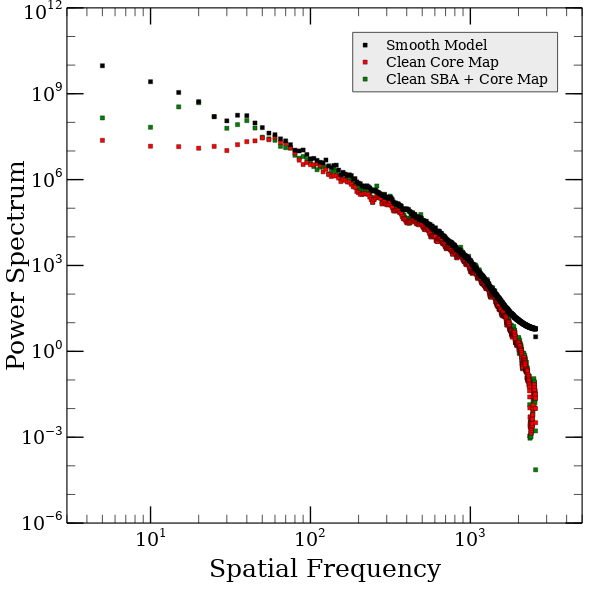
\includegraphics[width=0.49\columnwidth]{figs54/psd1_revised.png}
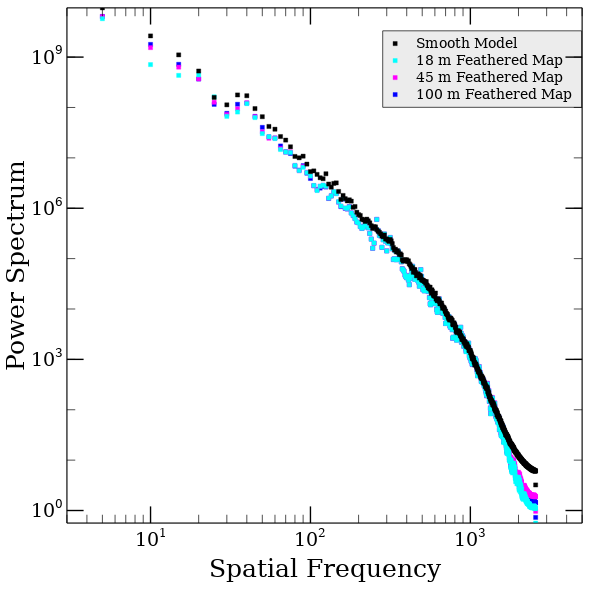
\includegraphics[width=0.49\columnwidth]{figs54/psd2_revised.png}
\caption{Power spectrum density as compared to the smoothed input model (black squares). The left figure shows the power spectrum for the cleaned image with just the ngVLA Core (red) and the cleaned image with both the short baseline array and the core (green). The right figure shows the total power and interferometric feathered images for each single-dish tested: \SI{18}{\meter} dish (cyan), \SI{45}{\meter} dish (magenta), and \SI{100}{\meter} dish (blue).}
\label{fig:psd}
\end{figure}





\end{document}
